\documentclass[../../main.tex]{subfiles}
\graphicspath{{../../image/}{../../figure/}}
\begin{document}

\section{真非线性系统的 Glimm 泛函}\label{section:ch13-glimm泛函}

此处的目标是估计近似解 $U_h$ 沿某些曲线的总变差界。我们仍在每个特征族要么真非线性、要么线性退化的假设下工作。

与 $U_h$ 相联系的\emph{网格曲线}（mesh curve）是一条折线，其顶点构成有限采样点列 $(y_{s_1}^{r_1},t_{s_1}),\cdots,(y_{s_m}^{r_m},t_{s_m})$，其中 $r_{\ell+1}=r_\ell+1$，且 $s_{\ell+1}=s_\ell-1$ 或 $s_{\ell+1}=s_\ell+1$（见\cref{figure:ch13-网格曲线}）。因而任意网格曲线 $I$ 的边也是上一节所考察的菱形区域的边。凡通过与网格曲线 $I$ 共享的边进入菱形的波，称为\emph{穿越} $I$。

当 $J\setminus I$ 是某个菱形（设为 $\Delta_s^r$）的上边界（即``西北''与``东北''边界）、而 $I\setminus J$ 是该菱形的下边界（即``西南''与``东南''边界）时，称网格曲线 $J$ 为网格曲线 $I$ 的\emph{直接后继}。于是 $J$ 与 $I$ 有相同的顶点，除一个 $(y_{s-1}^r,t_{s-1})$ 被替换为 $(y_{s+1}^r,t_{s+1})$。这在网格曲线族上诱导出一个自然偏序：当存在有限网格曲线列 $I=I_0,I_1,\cdots,I_m=J$，使 $I_\ell$ 是 $I_{\ell-1}$ 的直接后继（$\ell=1,\cdots,m$）时，称 $J$ 是 $I$ 的后继，记为 $I<J$。

\begin{figure}[ht]
\centering
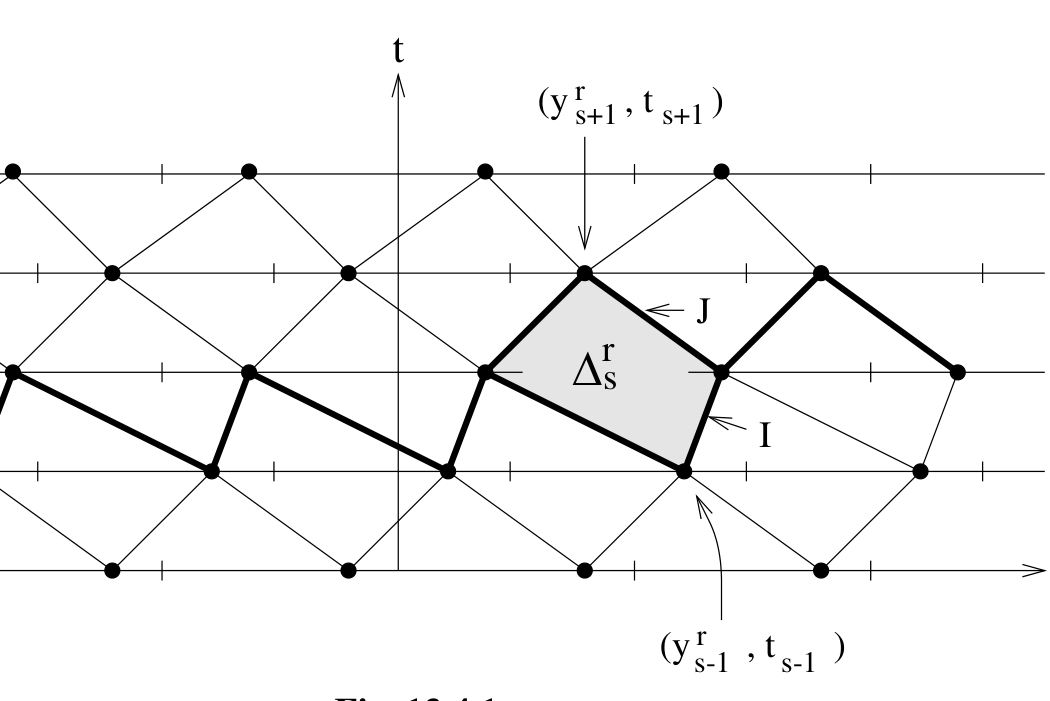
\includegraphics[width=0.85\textwidth]{ch13-fig04-01.png}
\caption{网格曲线 $I,J$ 与菱形 $\Delta_s^r$}\label{figure:ch13-网格曲线}
\end{figure}

与网格曲线 $I$ 相联系，定义泛函
\begin{align}
\mathscr{S}(I)&=\max|\xi|,\label{align:ch13-S-def}\\
\mathscr{L}(I)&=\sum|\xi|,
\label{align:ch13-L-def}
\end{align}
其中最大值与求和均遍历穿越 $I$ 的所有波的振幅 $\xi$。显然，$\mathscr{S}(I)$ 度量 $I$ 上 $U_h$ 的振幅，$\mathscr{L}(I)$ 度量沿曲线 $I$ 上 $U_h$ 的总变差。我们将通过监测从 $I$ 到其后继时 $\mathscr{S}$ 与 $\mathscr{L}$ 的变化，来估计 $U_h$ 的上确界与总变差。

设 $J$ 是 $I$ 的直接后继，如\cref{figure:ch13-网格曲线}所示。波扇 $\alpha=(\alpha_1,\cdots,\alpha_n)$ 与 $\beta=(\beta_1,\cdots,\beta_n)$ 分别通过 $\Delta_s^r$ 的``西南''边与``东南''边进入，并按\cref{section:ch13-真非线性波相互作用}中的讨论相互作用，产生波扇 $\varepsilon=(\varepsilon_1,\cdots,\varepsilon_n)$，通过``西北''边与``东北''边离开 $\Delta_s^r$。由\eqref{align:ch13-int-main}推出
\begin{align}
\mathscr{S}(J)&\leqslant\mathscr{S}(I)+[c_3+c_4\mathscr{S}(I)]\mathscr{D}(\Delta_s^r),\label{align:ch13-S-change}\\
\mathscr{L}(J)&\leqslant\mathscr{L}(I)+[c_3+c_4\mathscr{S}(I)]\mathscr{D}(\Delta_s^r),
\label{align:ch13-L-change}
\end{align}
其中 $c_3,c_4$ 也是\eqref{align:ch13-int-main}中的常数。特别地，当系统配备 Riemann 不变量坐标系时 $c_3=0$。显然，从 $I$ 推进到 $J$ 时 $\mathscr{S}$ 与 $\mathscr{L}$ 可能增大，因而仅凭\eqref{align:ch13-S-change}与\eqref{align:ch13-L-change}不足以得到所需的界\eqref{align:ch13-h-sup}、\eqref{align:ch13-h-tv}。

挽救局面的是这样一种认识：$\mathscr{L}$ 的增大只能由趋近波之间的相互作用所致，而这些波在交叉路径后便相互分离，永不再相遇。因此，未来相互作用的可能性蕴含于波的初始排列中，因而可预先估计。为把上述启发式论证形式化，我们将与网格曲线 $I$ 相联系一个泛函 $\mathscr{Q}(I)$，它度量穿越 $I$ 的波的\emph{未来相互作用势}。

穿越网格曲线 $I$ 的一个 $i$ 波与一个 $j$ 波称为\emph{趋近的}，若：(a) $i>j$ 且 $i$ 波在 $j$ 波之左穿越 $I$；或 (b) $i<j$ 且 $i$ 波在 $j$ 波之右穿越 $I$；或 (c) $i=j$，$i$ 特征族真非线性且两波中至少一个为激波。读者应注意它与\cref{chapter:ch09-容许波扇与riemann问题}中引入的两个相互作用波扇中趋近波概念的类似。
准备就绪后，令
\begin{align}
\mathscr{Q}(I)=\sum_{\mathrm{app}}|\zeta||\xi|,
\label{align:ch13-Q-def}
\end{align}
其中求和遍历穿越 $I$ 的所有趋近波对，$\zeta,\xi$ 为其振幅。显然，
\begin{align}
\mathscr{Q}(I)\leqslant\frac12[\mathscr{L}(I)]^2.
\label{align:ch13-Q-bound}
\end{align}

从网格曲线 $I$ 推进到其直接后继 $J$（如\cref{figure:ch13-网格曲线}所示）时，未来波相互作用势的变化由下述估计控制：
\begin{align}
\mathscr{Q}(J)-\mathscr{Q}(I)\leqslant\big\{[c_3+c_4\mathscr{S}(I)]\mathscr{L}(I)-1\big\}\mathscr{D}(\Delta_s^r),
\label{align:ch13-Q-change}
\end{align}
其中 $c_3,c_4$ 与\eqref{align:ch13-S-change}、\eqref{align:ch13-L-change}中相同。

为验证\eqref{align:ch13-Q-change}，我们区分\emph{外围波}（peripheral waves）与\emph{主体波}（principal waves）：前者同时穿越 $I$ 与 $J$，位于 $(y_s^{r-1},t_s)$ 之左或 $(y_s^{r+1},t_s)$ 之右；后者即波扇 $\alpha,\beta,\varepsilon$ 的组成部分，通过 $(y_s^{r-1},t_s)$ 与 $(y_s^{r+1},t_s)$ 之间穿越 $I$ 或 $J$。

首先注意到，入射波扇 $\alpha$ 与 $\beta$ 中主体波的相互作用向 $\mathscr{Q}(I)$ 贡献量 $\mathscr{D}(\Delta_s^r)$。相反，出射波扇 $\varepsilon$ 中没有哪一对主体波是趋近的，因而不对 $\mathscr{Q}(J)$ 作贡献。

其次注意到，外围波对向 $\mathscr{Q}(I)$ 与 $\mathscr{Q}(J)$ 的贡献相等；因而它们对 $\mathscr{Q}(J)-\mathscr{Q}(I)$ 的净贡献为零。

剩下须讨论外围波与主体波的配对。考察某个固定外围 $i$ 波（振幅 $\zeta$）与 $\alpha,\beta,\varepsilon$ 中 $j$ 波的配对对 $\mathscr{Q}(I)$ 与 $\mathscr{Q}(J)$ 的贡献。如真非线性情形所做，须区分如下情形：(i) $j>i$ 且外围 $i$ 波在 $(y_s^{r-1},t_s)$ 之左穿越 $I$；(ii) $j<i$ 且外围 $i$ 波在 $(y_s^{r+1},t_s)$ 之右穿越 $I$；(iii) $j>i$ 且外围 $i$ 波在 $(y_s^{r+1},t_s)$ 之右穿越 $I$；(iv) $j<i$ 且外围 $i$ 波在 $(y_s^{r-1},t_s)$ 之左穿越 $I$；(v) $j=i$，$\alpha_i\beta_i>0$ 且 $\zeta(\alpha_i+\beta_i)<0$；(vi) $j=i$，$\alpha_i\beta_i<0$ 且 $\zeta(\alpha_i+\beta_i)<0$；(vii) $j=i$，$\alpha_i\beta_i>0$ 且 $\zeta(\alpha_i+\beta_i)>0$。

在情形 (i)、(ii) 与 (iii) 中，外围 $i$ 波不与 $\alpha,\beta,\varepsilon$ 中任何 $j$ 波趋近；因而对 $\mathscr{Q}(I)$ 与 $\mathscr{Q}(J)$ 的贡献均为零。相反，在情形 (iv)、(v) 与 (vi) 中，外围 $i$ 波与 $\alpha,\beta,\varepsilon$ 中所有三个 $j$ 波趋近；因而对 $\mathscr{Q}(I)$ 与 $\mathscr{Q}(J)$ 的贡献分别为 $|\zeta|(|\alpha_j|+|\beta_j|)$ 与 $|\zeta||\varepsilon_j|$。

在其余情形 (vii) 中，视 $\alpha_i,\beta_i,\varepsilon_i$ 的符号而定，外围 $i$ 波可能与 $\alpha,\beta,\varepsilon$ 中全部、部分或不与任何 $i$ 波趋近；对 $\mathscr{Q}(I)$ 与 $\mathscr{Q}(J)$ 的贡献分别为 $\zeta(\alpha_i^-+\beta_i^-)$ 与 $\zeta\varepsilon_i^-$，其中上标``$-$''表示``负部''。

由上述及\eqref{align:ch13-int-main}，振幅为 $\zeta$ 的外围波与所有主体波配对对 $\mathscr{Q}(J)-\mathscr{Q}(I)$ 的总贡献不超过量 $|\zeta|[c_3+c_4\mathscr{S}(I)]\mathscr{D}(\Delta_s^r)$。因此我们断定，此类相互作用对 $\mathscr{Q}(J)-\mathscr{Q}(I)$ 的总贡献被 $[c_3+c_4\mathscr{S}(I)]\mathscr{L}(I)\mathscr{D}(\Delta_s^r)$ 控制。这就证明了\eqref{align:ch13-Q-change}。

\eqref{align:ch13-Q-change} 的关键推论是：当 $\mathscr{L}(I)$ 充分小时，从网格曲线 $I$ 推进到其直接后继 $J$ 时，未来波相互作用势 $\mathscr{Q}$ 减小。我们将利用这一性质来补偿 $\mathscr{S}$ 与 $\mathscr{L}$ 可能按\eqref{align:ch13-S-change}、\eqref{align:ch13-L-change}所允许的增大。为此，与网格曲线 $I$ 相联系，定义 Glimm 泛函
\begin{align}
\mathscr{G}(I)=\mathscr{L}(I)+2\kappa\mathscr{Q}(I),
\label{align:ch13-G-def}
\end{align}
其中 $\kappa$ 是 $c_3+c_4\mathscr{S}(I)$ 的某个固定上界，与 $I$ 和 $h$ 无关。尽管 $\mathscr{G}$ 控制 $\mathscr{L}$，但由\eqref{align:ch13-Q-bound}，它实际上与 $\mathscr{L}$ 等价。

\begin{theorem}[Glimm 泛函的递减性]\label{theorem:ch13-glimm递减}
设 $I$ 是满足 $2\kappa\mathscr{L}(I)\leqslant1$ 的网格曲线。则对 $I$ 的任意后继网格曲线 $J$，
\begin{align}
\mathscr{G}(J)&\leqslant\mathscr{G}(I),\label{align:ch13-G-dec}\\
\mathscr{L}(J)&\leqslant2\mathscr{L}(I).
\label{align:ch13-L-double}
\end{align}
进而，夹在曲线 $I$ 与 $J$ 之间的菱形中的波相互作用量与波抵消量有界：
\begin{align}
\sum\mathscr{D}(\Delta_s^r)&\leqslant[\mathscr{L}(I)]^2,\label{align:ch13-D-sum}\\
\sum\mathscr{C}(\Delta_s^r)&\leqslant\mathscr{L}(I).
\label{align:ch13-C-sum}
\end{align}
\end{theorem}

\begin{proof}
先设 $J$ 是如\cref{figure:ch13-网格曲线}所示的 $I$ 的直接后继。把\eqref{align:ch13-G-def}与\eqref{align:ch13-L-change}、\eqref{align:ch13-Q-change}结合，推出
\begin{align}
\mathscr{G}(J)\leqslant\mathscr{G}(I)+\kappa[2\kappa\mathscr{L}(I)-1]\mathscr{D}(\Delta_s^r).
\label{align:ch13-G-recur}
\end{align}
由于 $2\kappa\mathscr{L}(I)\leqslant1$，\eqref{align:ch13-G-recur}给出\eqref{align:ch13-G-dec}。进而，由\eqref{align:ch13-G-def}、\eqref{align:ch13-Q-bound}与 $2\kappa\mathscr{L}(I)\leqslant1$，得到
\begin{align}
\mathscr{G}(I)\leqslant2\mathscr{L}(I).
\label{align:ch13-G-twoL}
\end{align}
现设 $J$ 是 $I$ 的任意后继。迭代上述论证，同样可建立\eqref{align:ch13-G-dec}。由于 $\mathscr{L}(J)\leqslant\mathscr{G}(J)$，由\eqref{align:ch13-G-dec}与\eqref{align:ch13-G-twoL}得\eqref{align:ch13-L-double}。把\eqref{align:ch13-Q-change}对夹在 $I,J$ 之间的所有菱形求和，并利用\eqref{align:ch13-L-double}，得到
\begin{align}
\frac12\sum\mathscr{D}(\Delta_s^r)\leqslant\mathscr{Q}(I)-\mathscr{Q}(J),
\label{align:ch13-D-sum-intermediate}
\end{align}
由\eqref{align:ch13-Q-bound}即得\eqref{align:ch13-D-sum}。

把\eqref{align:ch13-cancel-est}对夹在曲线 $I,J$ 之间的所有菱形求和，得到
\begin{align}
2\sum\mathscr{C}(\Delta_s^r)\leqslant\mathscr{L}(I)-\mathscr{L}(J)+\kappa\sum\mathscr{D}(\Delta_s^r).
\label{align:ch13-C-sum-intermediate}
\end{align}
把\eqref{align:ch13-C-sum-intermediate}与\eqref{align:ch13-L-double}、\eqref{align:ch13-D-sum}结合，即得\eqref{align:ch13-C-sum}。证毕。
\end{proof}

上述定理具有根本重要性。特别地，估计\eqref{align:ch13-G-dec}与\eqref{align:ch13-L-double}提供了所需的总变差界，而\eqref{align:ch13-D-sum}与\eqref{align:ch13-C-sum}体现了非线性的耗散效应，对解的正则性与大时间行为有重要含义。

上述定理中的假设 $2\kappa\mathscr{L}(I)\leqslant1$ 意味着，对一般系统而言 $\mathscr{L}(I)$ 本身应充分小。然而，在配备 Riemann 不变量坐标系、$c_3=0$ 的系统中，只需 $\big(\sup U_h\big)\mathscr{L}(I)$ 充分小即可。对此特殊类系统，$\sup U_h$ 将借助下一定理估计。

\begin{theorem}[上确界的指数界]\label{theorem:ch13-sup指数界}
假设系统配备 Riemann 不变量坐标系。设 $I$ 是满足 $2\kappa\mathscr{L}(I)\leqslant1$ 的网格曲线。则对 $I$ 的任意后继网格曲线 $J$，
\begin{align}
\mathscr{S}(J)\leqslant\exp[c_4\mathscr{L}(I)^2]\,\mathscr{S}(I).
\label{align:ch13-S-exp}
\end{align}
\end{theorem}

\begin{proof}
先设 $J$ 是如\cref{figure:ch13-网格曲线}所示的 $I$ 的直接后继。由于 $c_3=0$，\eqref{align:ch13-S-change}给出
\begin{align}
\mathscr{S}(J)\leqslant[1+c_4\mathscr{D}(\Delta_s^r)]\mathscr{S}(I).
\label{align:ch13-S-recur}
\end{align}
迭代上述论证，可推出若 $J$ 是 $I$ 的任意后继，则
\begin{align}
\mathscr{S}(J)\leqslant\prod[1+c_4\mathscr{D}(\Delta_s^r)]\,\mathscr{S}(I),
\label{align:ch13-S-product}
\end{align}
其中乘积遍历夹在曲线 $I$ 与 $J$ 之间的所有菱形。把\eqref{align:ch13-S-product}与\eqref{align:ch13-D-sum}结合，即得\eqref{align:ch13-S-exp}。证毕。
\end{proof}

对于配备 Riemann 不变量坐标系的系统，宜用相应 Riemann 不变量的跳跃来度量波强度。特别地，对于激波曲线与稀疏波曲线重合的系统（见\cref{chapter:ch08-容许激波}），
这一策略使 $\mathscr{L}$ 从网格曲线到其后继保持非增，从而无需对初始数据总变差的大小作任何限制即可估计解的总变差。还有另一类非常特殊的两个守恒律系统，其中波强度的适当度量使 $\mathscr{L}$ 非增，从而在大总变差初始数据下 Cauchy 问题解亦存在。该类系统的一个有趣代表是系统
\begin{align}
\begin{cases}
\partial_t u-\partial_x v=0,\\
\partial_t v+\partial_x(u^{-1})=0,
\end{cases}
\label{align:ch13-isothermal}
\end{align}
即\cref{chapter:ch07-一维双曲平衡律组}取 $\sigma(u)=-u^{-1}$ 的特殊情形。
特别地，该系统描述了 Lagrangian 坐标下理想气体的等熵流。

\end{document}